%!TEX root = paper.tex

\section{The Common Fabric: Streaming Dataflows}
\label{sec:execution}

Although users can write Flink programs using a multitude of APIs, all Flink programs eventually compile down to a common representation: the dataflow graph. The dataflow graph is executed by Flink's runtime engine, the common layer underneath both the batch processing (DataSet) and stream processing (DataStream) APIs.

\subsection{Dataflow Graphs}
The dataflow graph, as depicted in \autoref{fig:dataflow}, is a directed acyclic graph (DAG) that consists of (i) stateful operators, and (ii) data streams that represent data produced by an operator and are available for consumption by operators. Since dataflow graphs are executed in a data-parallel fashion, operators are parallelized into one or more parallel instances called \emph{subtasks} and streams are split into one or more \emph{stream partitions} (one partition per producing subtask). 
The stateful operators (which may be stateless as a special case) implement all processing logic, e.g., filters, hash joins, stream window functions, etc. Many of these operators are implementations of textbook versions of well known algorithms. \autoref{sec:streaming} provides details on the implementation of windowing operators. Streams distribute data between producing and consuming operators in various patterns, such as point-to-point, broadcast, re-partition, fan-out, or merge.

\begin{figure}[t!]
\begin{minipage}{1.1\linewidth}
      \centering
       \hspace{-0.1\linewidth}
      \begin{minipage}{0.55\linewidth}
        \begin{figure}[H]
        \centering
        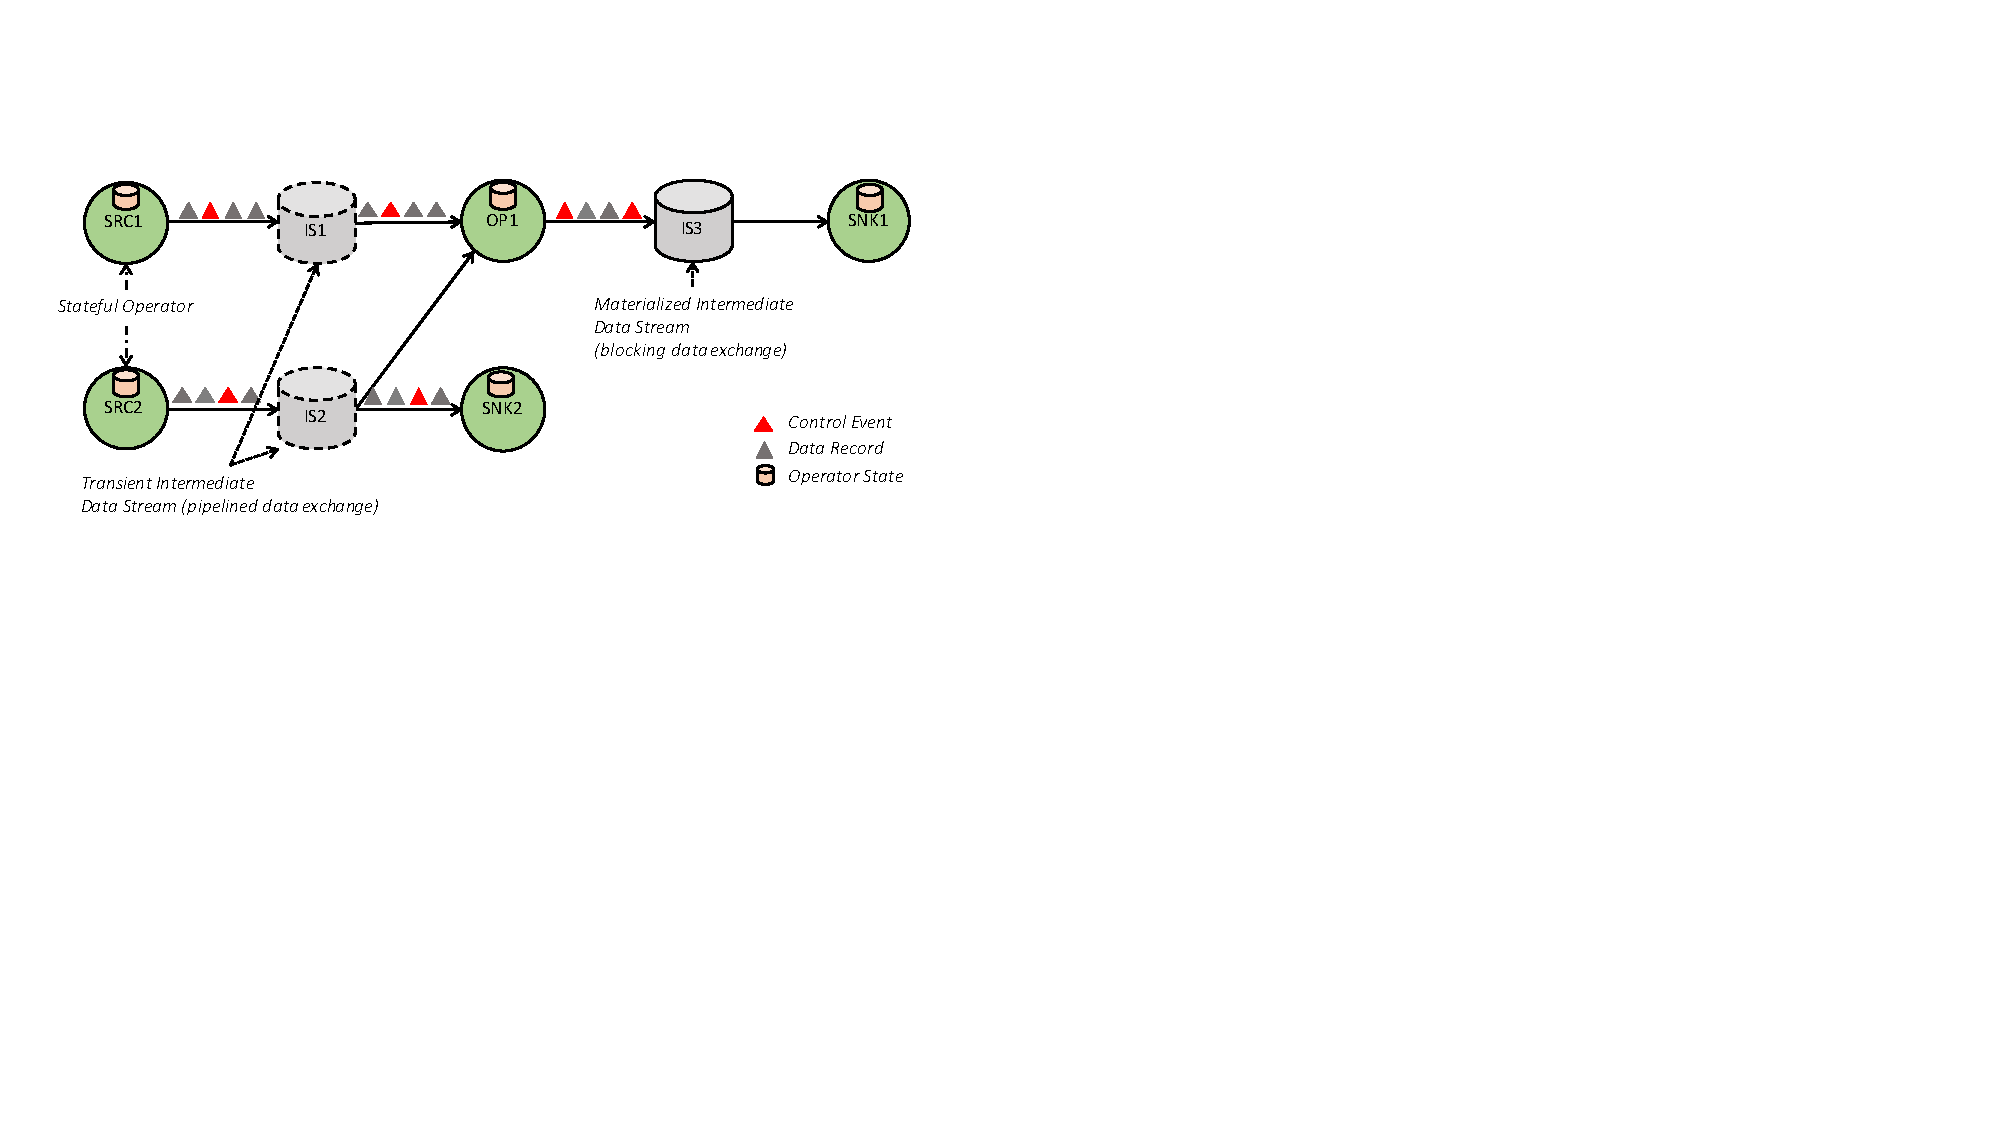
\includegraphics[width=.999\textwidth]{figs/dataflow}
        \vspace{-5mm}
        \caption{A simple dataflow graph.}
        \label{fig:dataflow}
        \end{figure}
      \end{minipage}
      
      \hspace{0.03\linewidth}
      % \vspace{-3mm}
      \begin{minipage}{0.32\linewidth}
          \begin{figure}[H]
				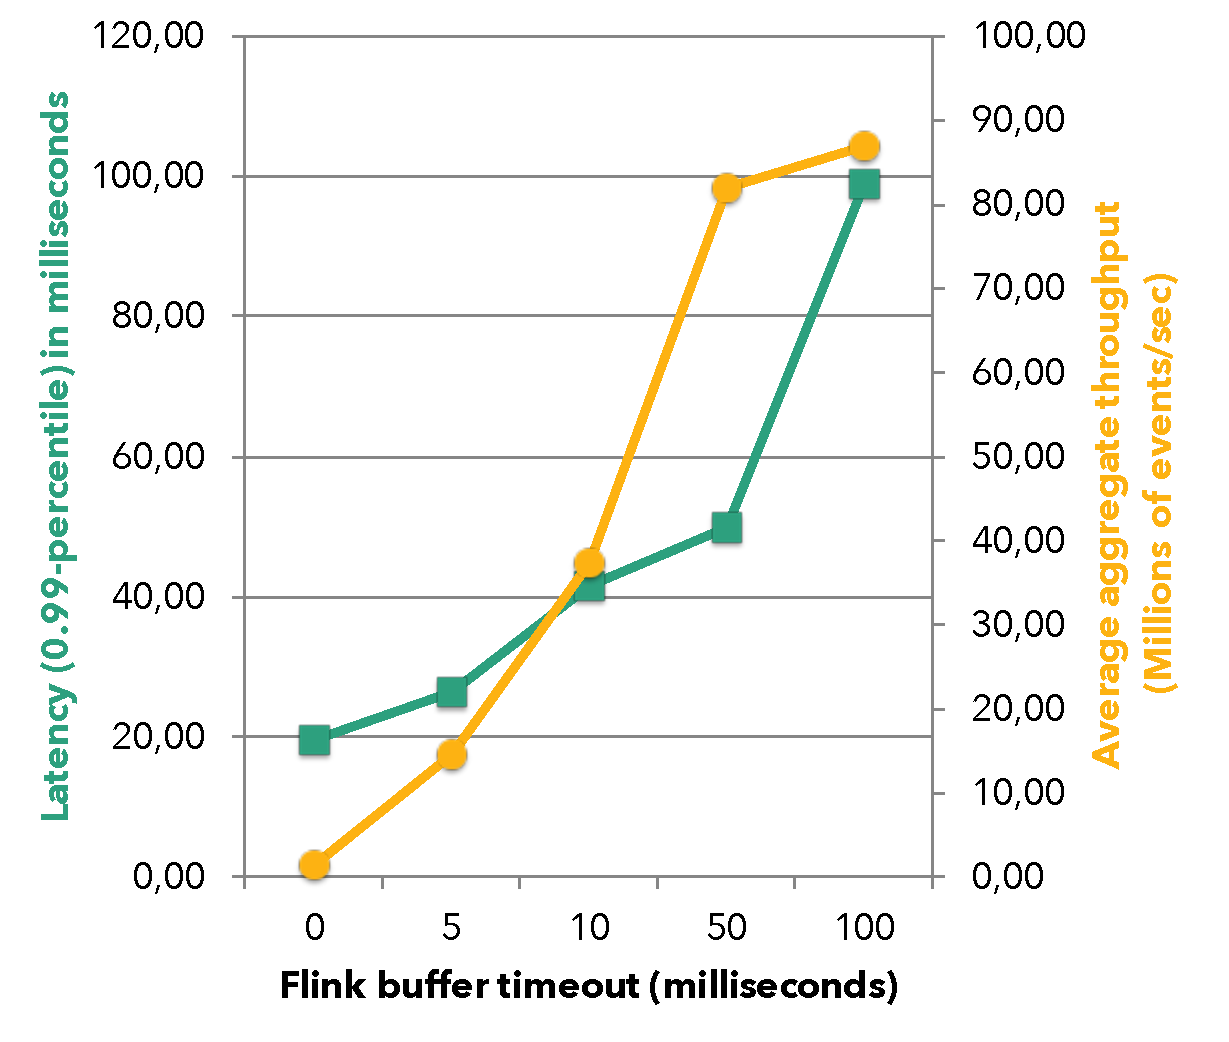
\includegraphics[width=.99\textwidth]{figs/latency-throughput.pdf}
				\vspace{-7mm}
    			\caption{The effect of buffer-timeout in latency and throughput.}
    			\label{fig:latency-throughput}
          \end{figure}
      \end{minipage}
  \end{minipage}
\end{figure}


\subsection{Data Exchange through Intermediate Data Streams}
Flink's intermediate data streams are the core abstraction for data exchange between operators. An intermediate data stream represents a logical handle to the data that is produced by an operator and can be consumed by one or more operators. Intermediate streams are logical in the sense that the data they point to may or may not be materialized on disk. The particular behavior of a data stream is parameterized by the higher layers in Flink (e.g., the program optimizer used by the DataSet API). 


\para{Pipelined and Blocking Data Exchange.} \emph{Pipelined intermediate streams} exchange data between concurrently running producers and consumers resulting in pipelined execution. As a result, pipelined streams propagate back pressure from consumers to producers, modulo some elasticity via intermediate buffer pools, in order to compensate for short-term throughput fluctuations. Flink uses pipelined streams for continuous streaming programs, as well as for many parts of batch dataflows, in order to avoid materialization when possible. \emph{Blocking streams}, on the other hand, are applicable to bounded data streams. A blocking stream buffers all of the producing operator's data before making it available for consumption, thereby separating the producing and consuming operators into different execution stages. Blocking streams naturally require more memory, frequently spill to secondary storage, and do not propagate backpressure. They are used to isolate successive operators against each other (where desired) and in situations where plans with pipeline-breaking operators such as joins, may cause distributed deadlocks.

\para{Balancing Latency and Throughput.} Flink’s data exchange mechanisms are implemented around the exchange of buffers. When a data record is ready on the producer side, it is serialized and split into one or more buffers that can be forwarded to consumers. A buffer is sent to a consumer either i) as soon as it is full, or ii) when a timeout condition is reached. This enables Flink to achieve high throughput by setting the size of buffers to a high value (e.g., a few kilobytes), as well as low latency by setting the buffer timeout to a low value (e.g., a few milliseconds). \autoref{fig:latency-throughput} shows the effect of buffer-timeouts to the throughput and latency of delivering records in a simple streaming grep job on 30 machines (120 cores). Flink can achieve an observable 99-th percentile latency of 20 milliseconds. The corresponding throughput is 24,500 events per second per core. As we increase the buffer timeout, we see an increase in latency with an increase in throughput, until full throughput is reached (where buffers fill up faster than the timeout expiration). At a buffer timeout of 50 milliseconds, the system reaches full throughput of 750,000 events per second per core with a 99-th percentile latency of 50 milliseconds.

\para{Control Events.} Apart from exchanging data, streams in Flink communicate different types of control events. These are special events injected in the data stream by operators, and are delivered in-order along with all other data records and events within a stream partition. The receiving operators react to these events by performing certain actions upon their arrival. Flink uses lots of special types of control events, including: \vspace{-2mm}
\begin{itemize}
\item \textit{Checkpoint barriers} that coordinate checkpoints by dividing the stream into pre-checkpoint and post-checkpoint (\autoref{sec:fault-tolerance}). \vspace{-3mm}
\item \textit{Watermarks} signaling the progress of event time within a stream partition (\autoref{sec:streaming-time}). \vspace{-3mm}
\item \textit{Iteration barriers} signaling that a stream partition has reached the end of a superstep, in Bulk/Stale-Synchronous-Parallel iterative algorithms on top of cyclic dataflows (\autoref{sec:batch-iterations}). \vspace{-1mm}
\end{itemize}

As mentioned above, control events assume that a stream partition preserves the order of records. To this end, unary operators in Flink consuming a single stream partition, \emph{guarantee a FIFO order of records}. However, operators receiving more than one stream partition merge the streams in arrival order, in order to keep up with the streams' rate and avoid back pressure. As a result, streaming dataflows in Flink do not provide ordering guarantees after any form of repartitioning or broadcasting, and the responsibility of dealing with out-of-order records is left to the operator implementation. We found that this gives the most efficient design, as most operators do not require deterministic order (e.g., hash-joins, maps, etc.), and operators that need to compensate for out-of-order arrivals (such as event time windows) can do that more efficiently as part of the operator logic.

\subsection{Fault Tolerance}
\label{sec:fault-tolerance}

Flink offers reliable execution with strict exactly-once-processing consistency guarantees and deals with failures via checkpointing and partial re-execution. The general assumption the system makes to effectively provide these guarantees is that the data sources are persistent and replayable. Examples of such sources are files and durable message queues (e.g. Apache Kafka). In practice, non-persistent sources can also be incorporated by keeping a look-ahead log within the state of the source operators.

The checkpointing mechanism of Apache Flink builds on the notion of distributed consistent snapshots/checkpoints to achieve exactly-once-processing guarantees. The possibly unbounded nature of a data stream makes re-computation upon recovery impractical, as possibly months of computation will need to be replayed considering a long running job. To bound recovery time, Flink takes a snapshot of the state of operators, including the current position of the input streams at regular intervals.

The core challenge lies in taking a consistent snapshot of all parallel operators without halting the execution of the topology. In essence, the snapshot of all operators should refer to the same logical time in the computation. The mechanism used in Flink is called Asynchronous Barrier Snapshotting, or ABS \cite{carbone2015lightweight}. Barriers are control records injected into the input streams that correspond to a logical time, and logically separate the stream to the part whose effects will be included in the current snapshot, and the part that will be snapshotted later.

\begin{figure}[t!]
	\centering
  	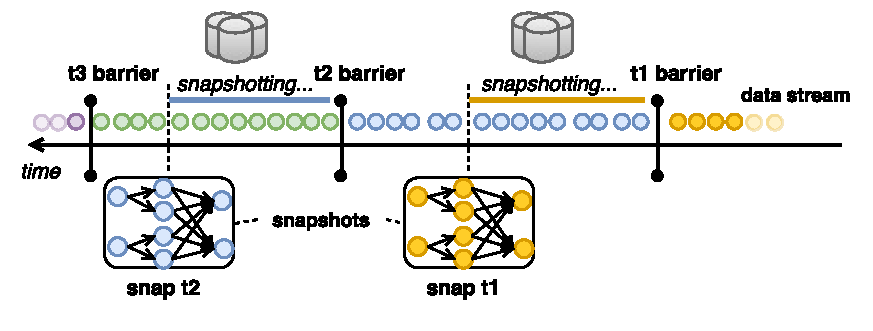
\includegraphics[width=.75\textwidth]{figs/snaps.pdf}
  	\vspace{-6mm}
	\caption{Asynchronous Barrier Snapshotting.}
	\vspace{-2mm}
	\label{fig:snapshots}
\end{figure}

An operator receives barriers from upstream and first performs an alignment phase, making sure that the barriers from all inputs have been received. Then, the operator writes its state (e.g., contents of a sliding window, or custom data structures) to durable storage (the storage backend can be an external system, e.g., HDFS). Once the state has been backed up, the operator forwards the barrier downstream. Eventually, all operators will register a snapshot of their state and a global snapshot will be complete. For example, in \autoref{fig:snapshots} we show that snapshot $t2$ contains all operator states that are the result of consuming all records before \emph{t2 barrier}. ABS bears resemblances to the seminal Chandy-Lamport algorithm for asynchronous distributed snapshots \cite{chandy1985distributed}. However, because of the DAG structure of a Flink program, ABS does not need to checkpoint in-flight records but solely rely on the aligning phase to apply all their effects to the operator states. This guarantees that the data that needs to be written to reliable storage is kept to the theoretical minimum (i.e., only the current state of the operators).

Recovery from failures reverts all operator states to their respective states taken from the last successful snapshot, and restarts the input streams starting from the latest barrier. The maximum amount of re-computation needed upon recovery is limited to the amount of input records between two consecutive barriers. Furthermore, partial recovery of a failed subtask is possible by additionally replaying unprocessed records  buffered at the immediate upstream subtasks \cite{carbone2015lightweight}.

\vspace{1mm}
\noindent ABS provides several benefits:\vspace{-2mm}
\begin{itemize}
\item It guarantees exactly-once state updates without ever pausing the computation \vspace{-3mm}
\item It is completely decoupled other forms of control messages, e.g., by events that trigger the computation of windows, thus not restricting the windowing mechanism to multiples of the checkpoint interval. \vspace{-3mm}
\item It is completely decoupled from the mechanism used for reliable storage, allowing state to be backed up to file systems, databases, etc, depending on the larger environment in which Flink is used.
\end{itemize}

\subsection{Iterative Dataflows}
\label{sec:iterations}

\begin{figure}[t!]
  \centering
    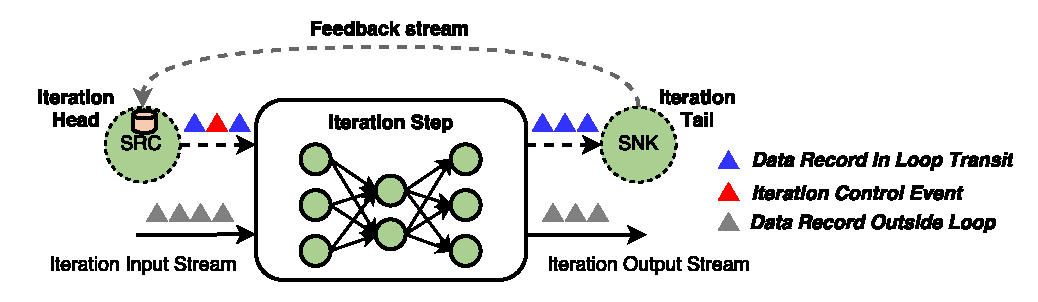
\includegraphics[width=.75\textwidth]{figs/iterations.pdf}
    \vspace{-6mm}
  \caption{The iteration model of Apache Flink}
  \vspace{-2mm}
  \label{fig:iterations}
\end{figure}

Loops and iterations are crucial for several applications. Support for iterations in data-intensive computing systems typically relies on submitting a new job for each iteration or by adding additional nodes to a running DAG \cite{DBLP:journals/pvldb/BuHBE10, DBLP:conf/hotcloud/ZahariaCFSS10}. Iterations in Flink are implemented as specialized operators that can contain other operators (iteration step) and can be part of the dag. As depicted in \autoref{fig:iterations}, Flink maintains the DAG-based runtime and scheduler, and allows for special iteration ``head'' and ``tail'' tasks that are implicitly connected with feedback edges. The role of these tasks is to establish an active feedback channel to the iteration step and provide coordination for processing data records in transit within this feedback channel. Coordination is needed for implementing any type of structured parallel iteration model such as the Bulk Synchronous Parallel (BSP) model as we explain in section \ref{sec:batch-iterations}. 
